\documentclass{standalone}
\usepackage{graphicx}	
\usepackage{amssymb, amsmath, amsthm}
\usepackage{color}
\usepackage{wasysym}

\usepackage{tikz}
\usetikzlibrary{math, calc}

\definecolor{light}{RGB}{220, 188, 188}
\definecolor{mid}{RGB}{185, 124, 124}
\definecolor{dark}{RGB}{143, 39, 39}
\definecolor{highlight}{RGB}{180, 31, 180}
\definecolor{lightteal}{RGB}{186, 219, 219}
\definecolor{midteal}{RGB}{124, 186, 186}
\definecolor{darkteal}{RGB}{38, 142, 142}
\definecolor{darkerteal}{RGB}{0, 124, 124}
\definecolor{gray10}{gray}{0.1}
\definecolor{gray20}{gray}{0.2}
\definecolor{gray30}{gray}{0.3}
\definecolor{gray40}{gray}{0.4}
\definecolor{gray60}{gray}{0.6}
\definecolor{gray70}{gray}{0.7}
\definecolor{gray80}{gray}{0.8}
\definecolor{gray90}{gray}{0.9}
\definecolor{gray95}{gray}{0.95}
  

\begin{document}

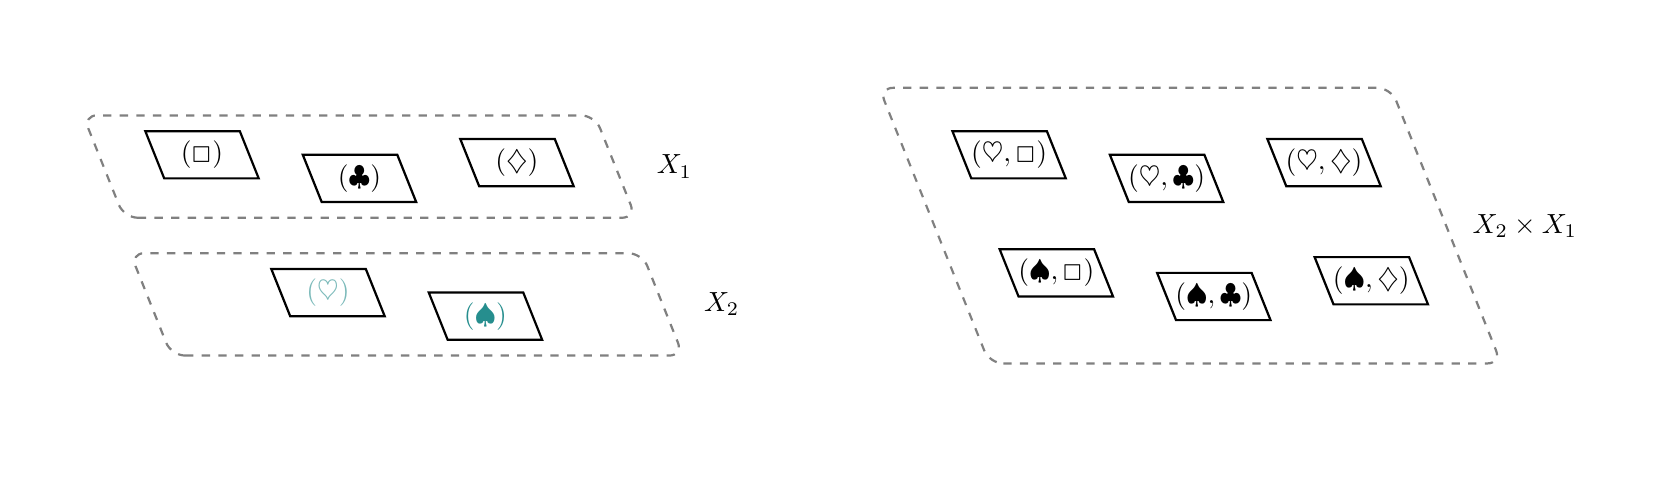
\begin{tikzpicture}[scale=1, thick]

  \begin{scope}[shift={(0, 0)}]
    \draw[white] (-4.5, -3) rectangle (5.75, 2.5);
    
    \pgfmathsetmacro{\dx}{0.6}
    \pgfmathsetmacro{\dy}{0.3}
    \pgfmathsetmacro{\tilt}{0.4}
    
    \begin{scope}[shift={(-2 - \tilt * 0.75, 0.15 + 0.75)}]
      \node at (0, 0) { $(\Box)$ };
      \draw[black]    ({-(1 - \tilt * \dy / \dx) * \dx}, -\dy) 
                   -- (+{(1 + \tilt * \dy / \dx) * \dx}, -\dy) 
                   -- ({+(1 - \tilt * \dy / \dx) * \dx}, +\dy) 
                   -- ({-(1 + \tilt * \dy / \dx) * \dx}, +\dy) -- cycle;
    \end{scope}
  
    \begin{scope}[shift={(+0 - \tilt * 0.75, -0.15 + 0.75)}]
      \node at (0, 0) { $(\clubsuit)$ };
      \draw[black]    ({-(1 - \tilt * \dy / \dx) * \dx}, -\dy) 
                   -- (+{(1 + \tilt * \dy / \dx) * \dx}, -\dy) 
                   -- ({+(1 - \tilt * \dy / \dx) * \dx}, +\dy) 
                   -- ({-(1 + \tilt * \dy / \dx) * \dx}, +\dy) -- cycle;
    \end{scope}
  
    \begin{scope}[shift={(+2 - \tilt * 0.75, +0.05 + 0.75)}]
      \node at (0, 0) { $(\diamondsuit)$ };
      \draw[black]    ({-(1 - \tilt * \dy / \dx) * \dx}, -\dy) 
                   -- (+{(1 + \tilt * \dy / \dx) * \dx}, -\dy) 
                   -- ({+(1 - \tilt * \dy / \dx) * \dx}, +\dy) 
                   -- ({-(1 + \tilt * \dy / \dx) * \dx}, +\dy) -- cycle;
    \end{scope}
  
    \begin{scope}[shift={(-1 + \tilt * 0.75, 0.15 - 1)}]
      \node[midteal] at (0, 0) { $(\heartsuit)$ };
      \draw[black]    ({-(1 - \tilt * \dy / \dx) * \dx}, -\dy) 
                   -- (+{(1 + \tilt * \dy / \dx) * \dx}, -\dy) 
                   -- ({+(1 - \tilt * \dy / \dx) * \dx}, +\dy) 
                   -- ({-(1 + \tilt * \dy / \dx) * \dx}, +\dy) -- cycle;
    \end{scope}
  
    \begin{scope}[shift={(+1 + \tilt * 0.75, -0.15 - 1)}]
      \node[darkteal] at (0, 0) { $(\spadesuit)$ };
      \draw[black]    ({-(1 - \tilt * \dy / \dx) * \dx}, -\dy) 
                   -- (+{(1 + \tilt * \dy / \dx) * \dx}, -\dy) 
                   -- ({+(1 - \tilt * \dy / \dx) * \dx}, +\dy) 
                   -- ({-(1 + \tilt * \dy / \dx) * \dx}, +\dy) -- cycle;
    \end{scope}
    
    \pgfmathsetmacro{\dx}{3.25}
    \pgfmathsetmacro{\dy}{0.65}
    
    \begin{scope}[shift={({-\tilt * 0.75}, 0.75)}]
      \draw[gray, dashed, rounded corners=5]   
           ({-(1 - \tilt * \dy / \dx) * \dx}, -\dy) 
        -- ({+(1 + \tilt * \dy / \dx) * \dx}, -\dy) 
        -- ({+(1 - \tilt * \dy / \dx) * \dx}, +\dy) 
        -- ({-(1 + \tilt * \dy / \dx) * \dx}, +\dy) -- cycle;
    \end{scope}
    
    \begin{scope}[shift={({+\tilt * 0.75}, -1)}]
      \draw[gray, dashed, rounded corners=5]   
           ({-(1 - \tilt * \dy / \dx) * \dx}, -\dy) 
        -- ({+(1 + \tilt * \dy / \dx) * \dx}, -\dy) 
        -- ({+(1 - \tilt * \dy / \dx) * \dx}, +\dy) 
        -- ({-(1 + \tilt * \dy / \dx) * \dx}, +\dy) -- cycle;
    \end{scope}
    
    \node[black] at (-\tilt * 0.75 + 4, +0.75) { $ X_{1}$ };
    \node[black] at (+\tilt * 0.75 + 4, -1) { $ X_{2}$ };
  \end{scope}
  
  \begin{scope}[shift={(10.25, 0)}]
    \draw[white] (-4.5, -3) rectangle (5.75, 2.5);
    
    \pgfmathsetmacro{\dx}{0.6}
    \pgfmathsetmacro{\dy}{0.3}
    \pgfmathsetmacro{\tilt}{0.4}
    
    \begin{scope}[shift={(-2 - \tilt * 0.75, 0.15 + 0.75)}]
      \node at (0, 0) { $(\heartsuit, \Box)$ };
      \draw[black]    ({-(1 - \tilt * \dy / \dx) * \dx}, -\dy) 
                   -- (+{(1 + \tilt * \dy / \dx) * \dx}, -\dy) 
                   -- ({+(1 - \tilt * \dy / \dx) * \dx}, +\dy) 
                   -- ({-(1 + \tilt * \dy / \dx) * \dx}, +\dy) -- cycle;
    \end{scope}
  
    \begin{scope}[shift={(+0 - \tilt * 0.75, -0.15 + 0.75)}]
      \node at (0, 0) { $(\heartsuit, \clubsuit)$ };
      \draw[black]    ({-(1 - \tilt * \dy / \dx) * \dx}, -\dy) 
                   -- (+{(1 + \tilt * \dy / \dx) * \dx}, -\dy) 
                   -- ({+(1 - \tilt * \dy / \dx) * \dx}, +\dy) 
                   -- ({-(1 + \tilt * \dy / \dx) * \dx}, +\dy) -- cycle;
    \end{scope}
  
    \begin{scope}[shift={(+2 - \tilt * 0.75, +0.05 + 0.75)}]
      \node at (0, 0) { $(\heartsuit, \diamondsuit)$ };
      \draw[black]    ({-(1 - \tilt * \dy / \dx) * \dx}, -\dy) 
                   -- (+{(1 + \tilt * \dy / \dx) * \dx}, -\dy) 
                   -- ({+(1 - \tilt * \dy / \dx) * \dx}, +\dy) 
                   -- ({-(1 + \tilt * \dy / \dx) * \dx}, +\dy) -- cycle;
    \end{scope}
  
    \begin{scope}[shift={(-2 + \tilt * 0.75, 0.15 - 0.75)}]
      \node at (0, 0) { $(\spadesuit, \Box)$ };
      \draw[black]    ({-(1 - \tilt * \dy / \dx) * \dx}, -\dy) 
                   -- (+{(1 + \tilt * \dy / \dx) * \dx}, -\dy) 
                   -- ({+(1 - \tilt * \dy / \dx) * \dx}, +\dy) 
                   -- ({-(1 + \tilt * \dy / \dx) * \dx}, +\dy) -- cycle;
    \end{scope}
  
    \begin{scope}[shift={(+0 + \tilt * 0.75, -0.15 - 0.75)}]
      \node at (0, 0) { $(\spadesuit, \clubsuit)$ };
      \draw[black]    ({-(1 - \tilt * \dy / \dx) * \dx}, -\dy) 
                   -- (+{(1 + \tilt * \dy / \dx) * \dx}, -\dy) 
                   -- ({+(1 - \tilt * \dy / \dx) * \dx}, +\dy) 
                   -- ({-(1 + \tilt * \dy / \dx) * \dx}, +\dy) -- cycle;
    \end{scope}
  
    \begin{scope}[shift={(+2 + \tilt * 0.75, +0.05 - 0.75)}]
      \node at (0, 0) { $(\spadesuit, \diamondsuit)$ };
      \draw[black]    ({-(1 - \tilt * \dy / \dx) * \dx}, -\dy) 
                   -- (+{(1 + \tilt * \dy / \dx) * \dx}, -\dy) 
                   -- ({+(1 - \tilt * \dy / \dx) * \dx}, +\dy) 
                   -- ({-(1 + \tilt * \dy / \dx) * \dx}, +\dy) -- cycle;
    \end{scope}
    
    \pgfmathsetmacro{\dx}{3.25}
    \pgfmathsetmacro{\dy}{1.75}
    
  
    \begin{scope}[shift={(0, 0)}]
      \draw[gray, dashed, rounded corners=5]   
           ({-(1 - \tilt * \dy / \dx) * \dx}, -\dy) 
        -- ({+(1 + \tilt * \dy / \dx) * \dx}, -\dy) 
        -- ({+(1 - \tilt * \dy / \dx) * \dx}, +\dy) 
        -- ({-(1 + \tilt * \dy / \dx) * \dx}, +\dy) -- cycle;
    \end{scope}
    
    \node[black] at (+\tilt * 0 + 4.25, 0) { $ X_{2} \times X_{1}$ };
  \end{scope}
  
\end{tikzpicture}

\end{document}  